This chapter will contain the background knowledge for the anatomy and physiology of the knee and the definition of pain. Furthermore is the pattern recognition described, where machine learning and deep learning are specified. 

\section{Anatomy and Physiology}
In this section are the anatomy of the knee and the definition of pain described to optimise the understanding of patellofemoral pain. 

\subsection{Knee}
The knee is the largest joint in the body and consists of a hinge and a gliding joint. The hinge joint is placed between the lateral and medial femoral condyles and the lateral and medial tibial condyles. Between the patella and femur is the gliding joint formed.\citep{Martini2012} 
There is three separate articulations in the knee joint, which is one between the patella and the patellar surface of the femur and two between the femoral and tibial condyles. Additionally, the knee consist of seven major ligaments that stabilize the knee joint, which are listed below and can be seen in \autoref{fig:knee}.\citep{Martini2012}

\begin{itemize}
\item The patellar ligament 
\item Two popliteal ligaments
\item The anterior cruciate ligament (ACI) and posterior cruciate ligament (PCI) 
\item The tibial collateral ligament and the fibular collateral ligament \citep{Martini2012}
\end{itemize}

\begin{figure} [H]
\centering
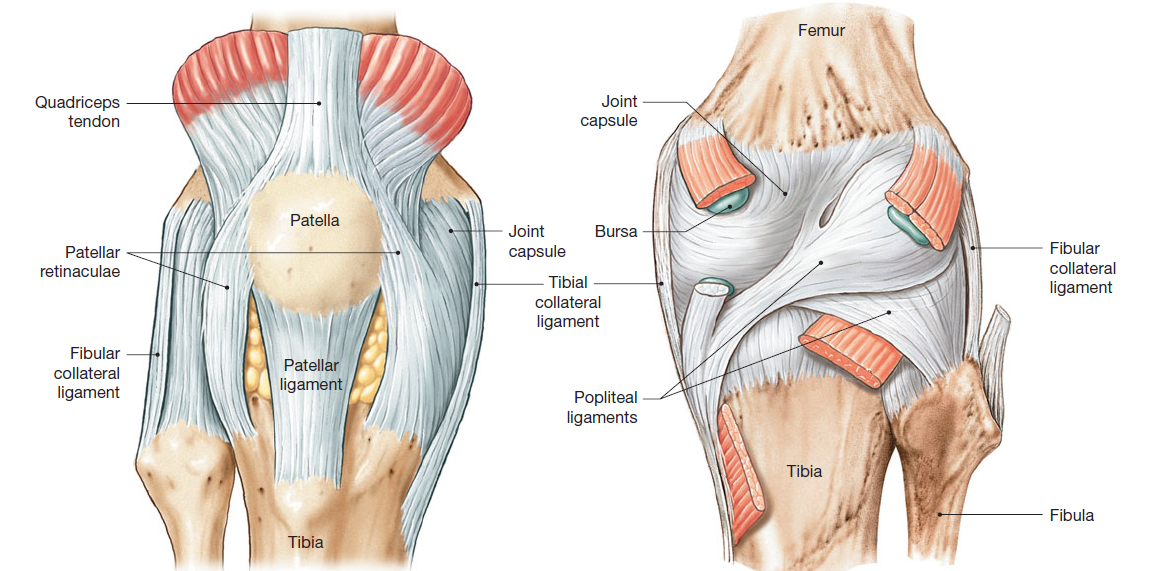
\includegraphics[width=1\textwidth]{figures/knee}
\caption{The figure illustrates the anatomy of the knee with focus on the ligaments. Edited from \citep{Martini2012}.}
\label{fig:knee}
\end{figure}


\subsection{Pain}
Pain is experienced and perceived subjectively and there is a lack of methods to measure pain accurately \citep{IASP2012, Younger2009}. 
The International Association for the Study of Pain (IASP) has defined pain as being “an unpleasant sensory and emotional experience associated with actual or potential tissue damage” \citep{IASP2012}.

Physiologically pain can be divided into three categories: Acute pain (less than three months), persistent or chronic pain and cancer pain. Furthermore, pain can be either nociceptive or neuropathic. Nociceptive pain is associated with tissue damage. Neuropathic is associated with damage to the nervous system.\citep{Briggs2010} 
